\section{Xây dựng và Triển khai Ứng dụng}

Sau khi lựa chọn và lượng tử hóa mô hình YOLO26-seg, nhóm xây dựng một ứng dụng Web hoàn chỉnh nhằm đưa kết quả nghiên cứu vào quy trình sử dụng thực tế. Hệ thống cho phép người dùng tải ảnh lá lúa hoặc cà phê, nhận kết quả chẩn đoán cùng độ tin cậy, xem các phương án mà mô hình đã cân nhắc và tham khảo hướng xử lý từ cơ sở tri thức chuyên gia. Ứng dụng được triển khai công khai tại \url{https://plant-disease-demo.duckdns.org/} trên một máy ảo Google Cloud Platform (GCP), sử dụng k3s để điều phối các dịch vụ.

\subsection{Kiến trúc Hệ thống}

\subsubsection{Kiến trúc tổng thể}

Hệ thống được tổ chức theo kiến trúc nhiều tầng để tách biệt giao diện, nghiệp vụ, suy luận và lưu trữ. Cách tổ chức này giúp mỗi thành phần có thể được đóng gói, cấu hình và triển khai độc lập. Hình~\ref{fig:ch5-deployment-architecture} trình bày đồng thời luồng truy cập từ người dùng, các workload bên trong cụm k3s và quy trình đưa phiên bản mới lên môi trường vận hành.

\begin{figure}[htbp]
  \centering
  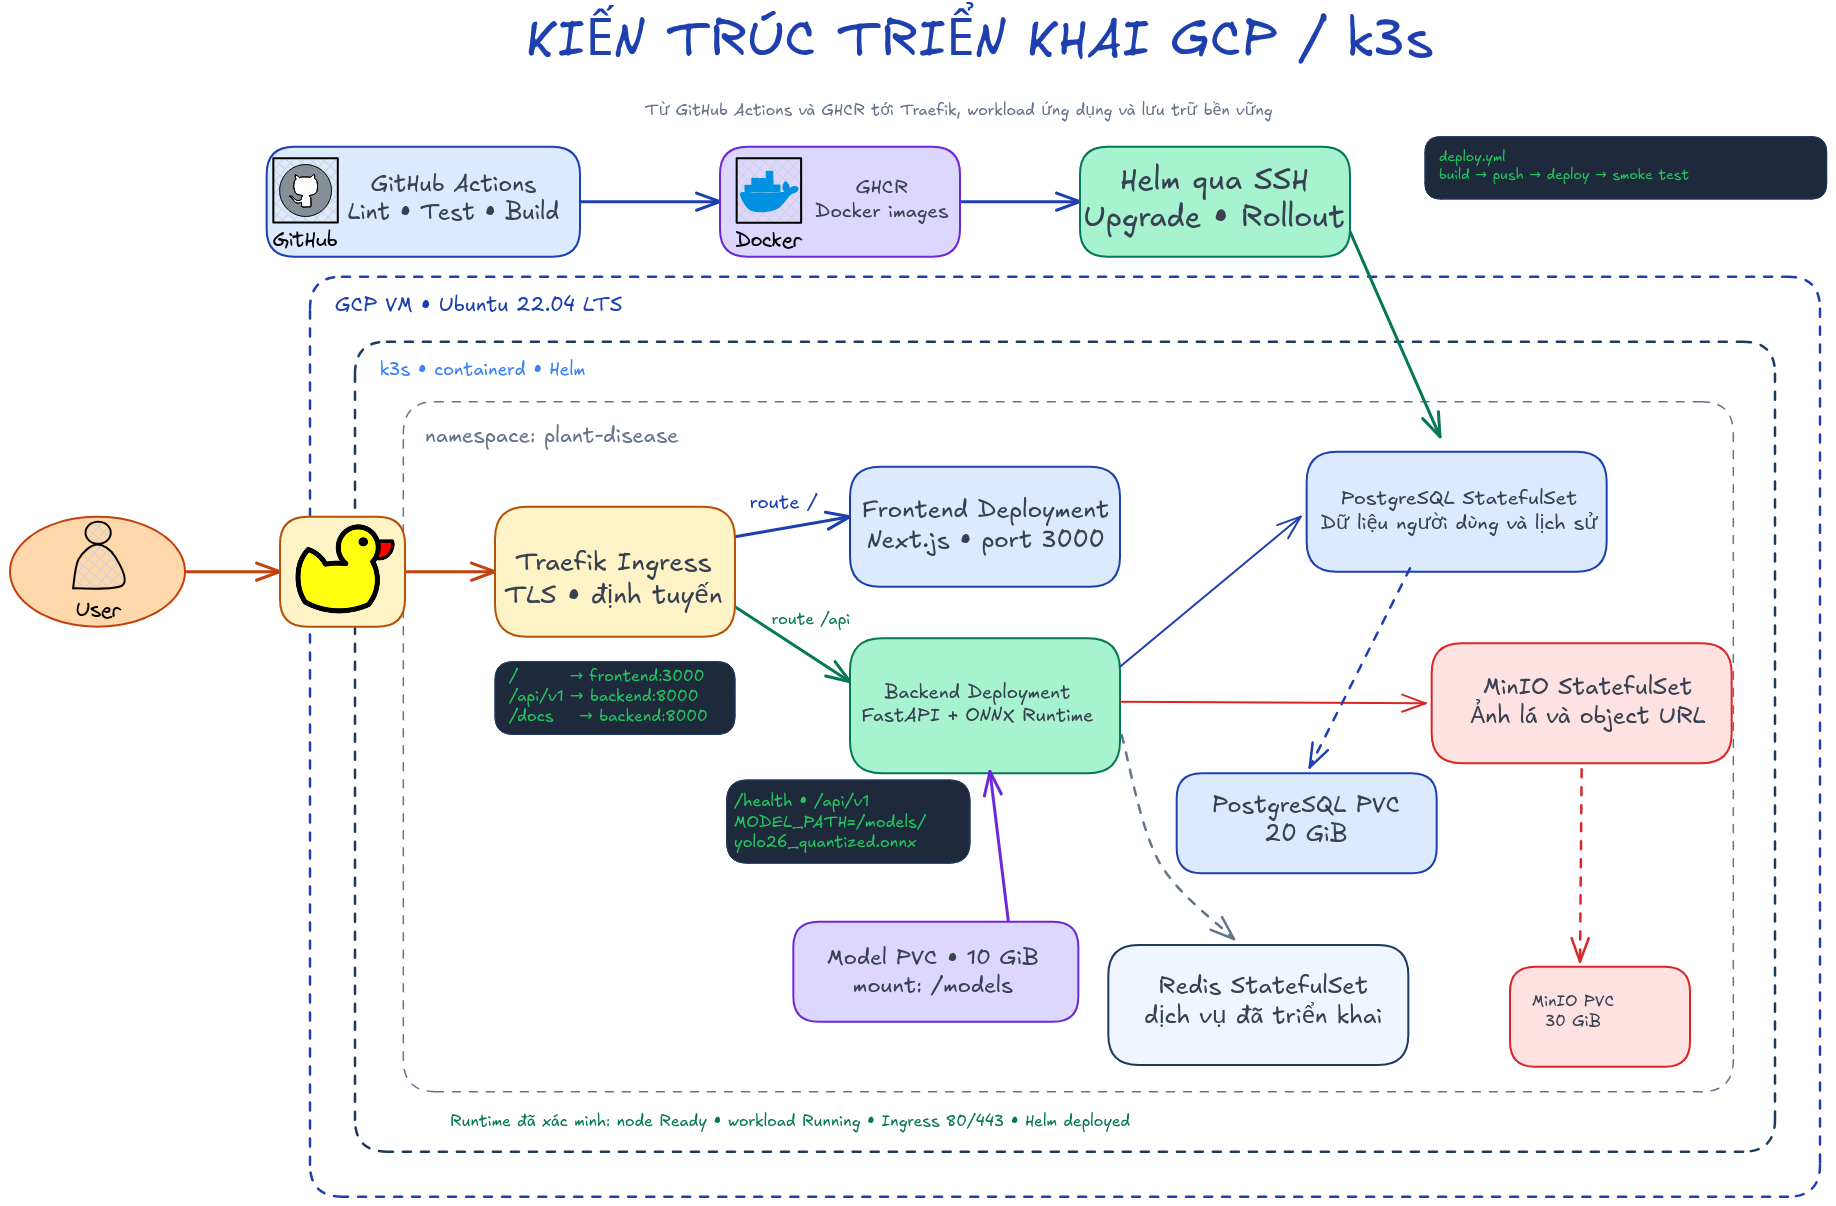
\includegraphics[width=\textwidth]{img/ch5/deployment-architecture-gcp-k3s.png}
  \caption{Kiến trúc triển khai ứng dụng trên GCP và k3s}
  \label{fig:ch5-deployment-architecture}
\end{figure}

Các thành phần chính và trách nhiệm tương ứng được tổng hợp trong Bảng~\ref{tab:ch5-system-components}.

\begin{table}[htbp]
  \centering
  \caption{Các thành phần chính trong kiến trúc ứng dụng}
  \label{tab:ch5-system-components}
  \small
  \begin{tabularx}{\textwidth}{|p{2.7cm}|p{3.0cm}|X|}
    \hline
    \textbf{Thành phần} & \textbf{Công nghệ} & \textbf{Vai trò} \\
    \hline
    Frontend & Next.js 15, React 19 & Cung cấp giao diện tải ảnh, hiển thị kết quả, đăng nhập, lịch sử và cơ sở tri thức. \\ \hline
    Backend API & FastAPI, Uvicorn & Kiểm tra yêu cầu, điều phối suy luận, xác thực, lưu lịch sử và trả dữ liệu JSON cho frontend. \\ \hline
    Dịch vụ suy luận & ONNX Runtime & Nạp mô hình \texttt{yolo26\_quantized.onnx}, tiền xử lý ảnh kích thước $640\times640$ và trả về năm nhãn có xác suất cao nhất. \\ \hline
    Cơ sở tri thức & JSON theo luật & Ánh xạ tám nhãn mô hình sang mô tả, triệu chứng, nguyên nhân, biện pháp xử lý, phòng bệnh và nguồn tham khảo tiếng Việt. \\ \hline
    Cơ sở dữ liệu & PostgreSQL 16 & Lưu tài khoản, metadata ảnh, nhãn dự đoán, độ tin cậy, top-$k$, khuyến nghị, phiên bản mô hình và độ trễ. \\ \hline
    Lưu trữ ảnh & MinIO & Lưu tệp ảnh trong bucket \texttt{plant-disease-images} và sinh URL có thời hạn để truy xuất ảnh. \\ \hline
    Điều phối & k3s, Helm, Traefik & Quản lý workload, cấu hình dịch vụ nội bộ, lưu trữ bền vững, định tuyến và HTTPS. \\ \hline
  \end{tabularx}
\end{table}

Frontend không truy cập trực tiếp mô hình hay tầng dữ liệu. Mọi thao tác nghiệp vụ đều đi qua REST API tại tiền tố \texttt{/api/v1}. Traefik chuyển các đường dẫn \texttt{/api/v1}, \texttt{/health}, \texttt{/docs}, \texttt{/redoc} và \texttt{/openapi.json} đến backend ở cổng 8000; đường dẫn gốc \texttt{/} được chuyển đến frontend ở cổng 3000. PostgreSQL, MinIO và Redis chỉ được công bố dưới dạng \texttt{ClusterIP}, do đó không mở trực tiếp ra Internet.

\subsubsection{Luồng chẩn đoán}

Luồng xử lý của một yêu cầu chẩn đoán gồm các bước sau:

\begin{enumerate}
  \item Người dùng chọn ảnh JPEG, PNG hoặc WebP trên giao diện. Backend kiểm tra kiểu nội dung, tệp rỗng và giới hạn dung lượng 10 MB trước khi suy luận.
  \item Endpoint \texttt{POST /api/v1/predict} đọc ảnh và gọi dịch vụ ONNX Runtime. Đối tượng suy luận được lưu trong bộ nhớ đệm tiến trình để tránh nạp lại mô hình ở mỗi yêu cầu.
  \item Mô hình trả về năm kết quả có độ tin cậy cao nhất. Backend ghi nhận thời gian suy luận và chọn kết quả đứng đầu làm nhãn chẩn đoán.
  \item Nhãn được ánh xạ sang bản ghi trong \texttt{backend/app/knowledge/diseases.json}. Phản hồi được bổ sung mô tả bệnh, triệu chứng, nguyên nhân, hướng xử lý, phòng ngừa và cảnh báo an toàn. Nếu độ tin cậy dưới 60\%, hệ thống khuyến nghị người dùng chụp lại ảnh rõ hơn và đối chiếu triệu chứng ngoài thực địa.
  \item Ảnh gốc được tải lên MinIO; metadata ảnh và kết quả dự đoán được ghi vào PostgreSQL trong cùng luồng nghiệp vụ. Nếu người dùng đã đăng nhập, bản ghi được liên kết với tài khoản để hiển thị trong lịch sử.
  \item Backend trả về nhãn, độ tin cậy, top-$5$, khuyến nghị, URL ảnh, mã bản ghi và độ trễ để frontend trình bày.
\end{enumerate}

Thiết kế cho phép khách chưa đăng nhập thực hiện chẩn đoán, trong khi endpoint \texttt{GET} \path{/api/v1/history} yêu cầu JSON Web Token (JWT). Token dùng thuật toán HS256 và có thời hạn mặc định 24 giờ trên môi trường triển khai. Redis đã được triển khai dưới dạng StatefulSet có lưu trữ bền vững để phục vụ khả năng mở rộng sau này; tuy nhiên, mã nghiệp vụ hiện tại chưa sử dụng Redis trong đường đi của yêu cầu chẩn đoán, vì vậy hệ thống không xem Redis là điều kiện để trả kết quả.

\subsection{Đóng gói và Tích hợp Mô hình}

\subsubsection{Tích hợp ONNX Runtime}

Checkpoint được xuất và lượng tử hóa thành tệp \path{models/yolo26_quantized.onnx}. Backend sử dụng ONNX Runtime~\cite{onnxruntime2026} thay vì phụ thuộc trực tiếp vào môi trường huấn luyện, nhờ đó giảm số lượng thư viện cần thiết và cho phép suy luận trên CPU của máy ảo. Tên lớp được đọc từ \path{/models/class_names.json}; biến môi trường \texttt{MODEL\_PATH} trỏ đến \path{/models/yolo26_quantized.onnx}. Phiên bản được lưu cùng mỗi lần chẩn đoán là \texttt{yolo26-seg-onnx}, giúp truy vết kết quả khi mô hình được nâng cấp.

Trên Kubernetes, thư mục \texttt{/models} của backend được gắn với PersistentVolumeClaim dung lượng 10 GiB. Init container kiểm tra sự tồn tại của tệp ONNX trước khi backend khởi động; nếu chưa có và cấu hình \texttt{MODEL\_DOWNLOAD\_URL} được cung cấp thì tệp được tải vào volume, ngược lại quản trị viên có thể nạp thủ công. Cách tách artifact mô hình khỏi vòng đời của pod giúp khởi động lại hoặc nâng cấp image ứng dụng mà không phải sao chép lại mô hình vào từng pod.

\subsubsection{Đóng gói ứng dụng bằng Docker}

Backend được xây dựng từ \texttt{python:3.12-slim}. Công cụ \texttt{uv} cài đặt chính xác các dependency từ lockfile; khi container khởi động, Alembic nâng cấp schema cơ sở dữ liệu trước khi Uvicorn phục vụ API trên cổng 8000. Liveness probe và readiness probe cùng gọi \texttt{/health}, cho phép Kubernetes phát hiện tiến trình lỗi và chỉ chuyển lưu lượng khi backend sẵn sàng.

Frontend sử dụng quy trình build nhiều giai đoạn trên \texttt{node:22-alpine}. Giai đoạn đầu cài dependency, giai đoạn thứ hai tạo production bundle của Next.js~\cite{nextjs2026}, và giai đoạn cuối chỉ chứa standalone server cùng tài nguyên tĩnh. Biến \texttt{NEXT\_PUBLIC\_API\_BASE\_URL} được truyền tại thời điểm build để frontend gọi đúng API công khai. Cách build này làm giảm nội dung dư thừa trong image chạy thực tế và giữ tách biệt dependency phát triển.

\subsection{Giao diện và Chức năng}

Giao diện được thiết kế theo hướng tối giản, ưu tiên quy trình chẩn đoán và khả năng đọc trên cả máy tính lẫn thiết bị di động. Thanh điều hướng cung cấp ba chức năng chính: tạo chẩn đoán mới, tra cứu cơ sở tri thức và xem lịch sử chẩn đoán. Hình~\ref{fig:ch5-home} cho thấy trang giới thiệu công khai cùng lời kêu gọi bắt đầu chẩn đoán.

\begin{figure}[htbp]
  \centering
  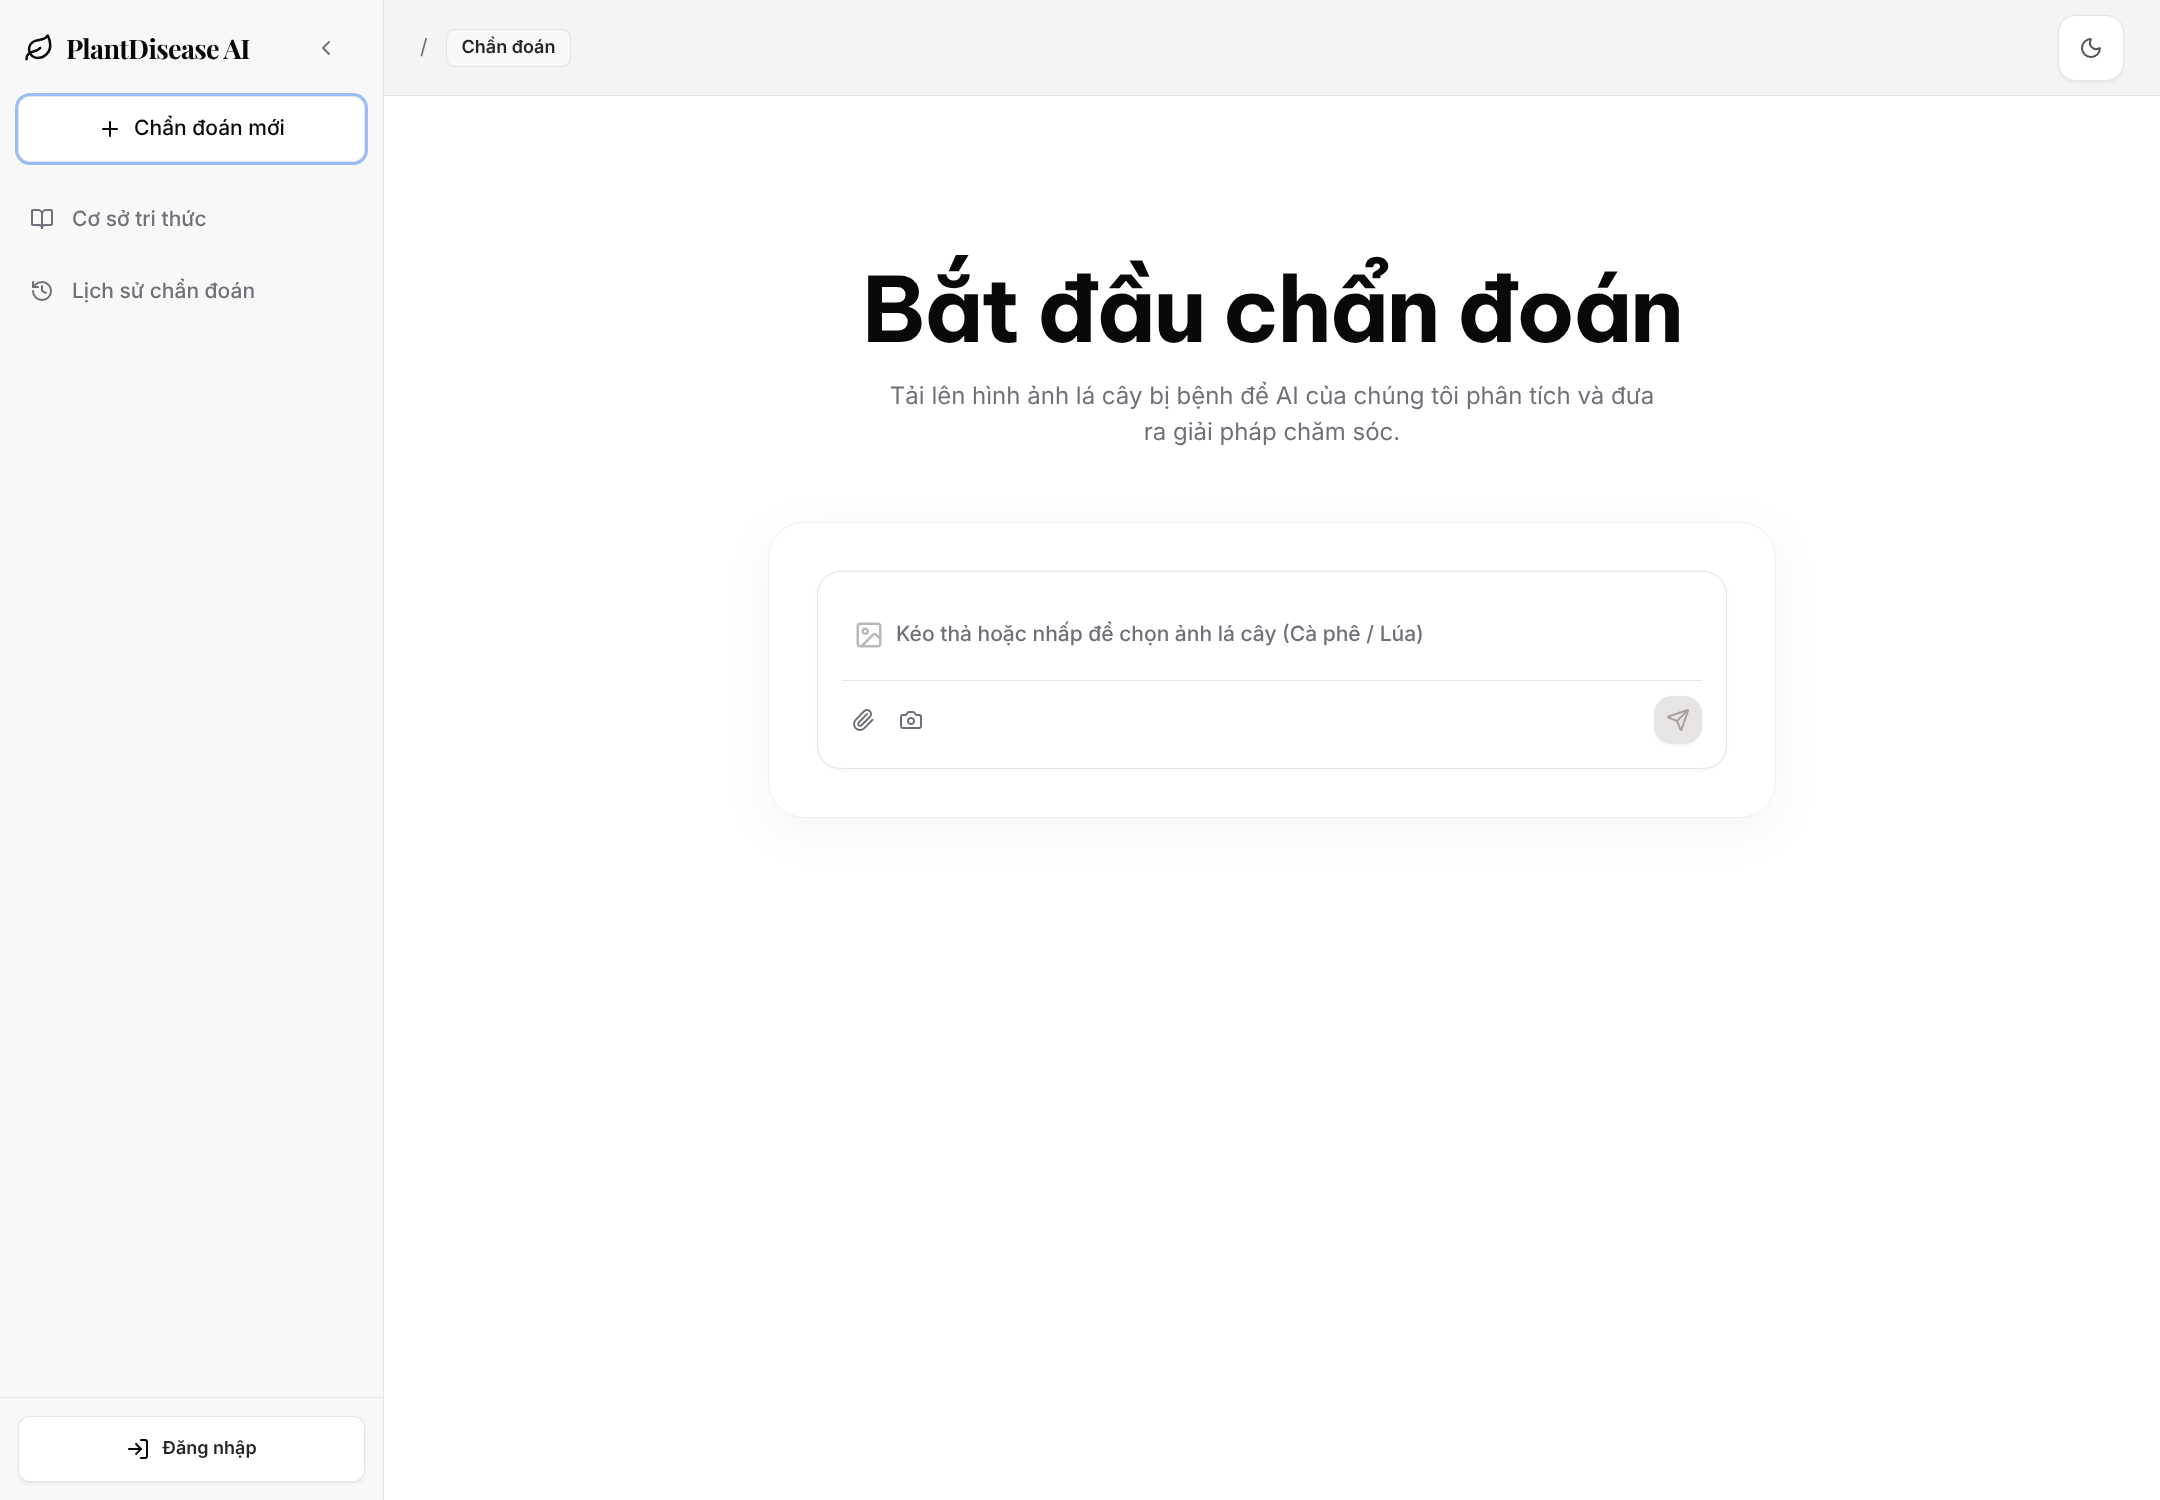
\includegraphics[width=\textwidth,height=0.78\textheight,keepaspectratio]{img/ch5/web-home.png}
  \caption{Trang chủ của ứng dụng PlantDisease AI}
  \label{fig:ch5-home}
\end{figure}

\subsubsection{Xác thực và lịch sử}

Người dùng có thể đăng ký hoặc đăng nhập để liên kết các lần chẩn đoán với tài khoản. Backend băm mật khẩu trước khi lưu, phát hành JWT sau khi đăng nhập và xác thực token đối với API lịch sử. Giao diện đăng nhập được minh họa trong Hình~\ref{fig:ch5-login}. Khách vẫn có thể thực hiện chẩn đoán nhanh, nhưng cần đăng nhập nếu muốn lưu và quản lý lịch sử cá nhân.

Luồng xử lý sau khi đăng nhập gồm các bước sau:

\begin{enumerate}
  \item Frontend gửi tên đăng nhập và mật khẩu đến API \texttt{POST /api/v1/auth/login}. Khi thông tin hợp lệ, backend trả về access token dạng JWT.
  \item Frontend lưu token trong bộ nhớ cục bộ của trình duyệt và gọi \texttt{GET /api/v1/auth/me} để xác minh phiên, đồng thời tải thông tin người dùng. Nút đăng nhập trên thanh bên được thay bằng menu tài khoản, trong đó hiển thị tên người dùng và chức năng đăng xuất.
  \item Khi người dùng gửi ảnh chẩn đoán, frontend đính kèm token vào tiêu đề \texttt{Authorization: Bearer}. Backend nhận diện người dùng hiện tại, lưu ảnh vào MinIO và ghi metadata ảnh cùng kết quả dự đoán vào PostgreSQL với \texttt{user\_id} tương ứng.
  \item Khi mở mục lịch sử, frontend gọi API \texttt{GET /api/v1/history} có phân trang. Backend chỉ truy vấn các bản ghi thuộc tài khoản đang đăng nhập; giao diện hiển thị ảnh thu nhỏ, cây trồng, tên bệnh, độ tin cậy và thời điểm chẩn đoán. Người dùng có thể mở rộng từng mục để xem khuyến nghị và chuyển giữa các trang kết quả.
  \item Khi tải lại trang, ứng dụng phục hồi token và kiểm tra lại hồ sơ người dùng. Nếu token hết hạn hoặc API trả về mã 401, phiên đăng nhập được xóa và giao diện yêu cầu đăng nhập lại. Thao tác đăng xuất cũng xóa token và dữ liệu người dùng khỏi trình duyệt.
\end{enumerate}

Như vậy, chuỗi xử lý chính có thể tóm tắt là: \textbf{đăng nhập $\rightarrow$ nhận JWT $\rightarrow$ xác minh hồ sơ $\rightarrow$ chẩn đoán có định danh $\rightarrow$ lưu MinIO/PostgreSQL $\rightarrow$ xem lịch sử cá nhân}. Cơ sở tri thức vẫn có thể được tra cứu công khai, còn JWT được dùng để bảo vệ dữ liệu lịch sử và tách biệt dữ liệu giữa các tài khoản.

Lịch sử hỗ trợ phân trang, hiển thị ảnh, nhãn dự đoán, độ tin cậy, top-$k$, khuyến nghị và thời điểm thực hiện; ảnh được truy xuất qua URL có thời hạn do MinIO sinh ra.

\begin{figure}[htbp]
  \centering
  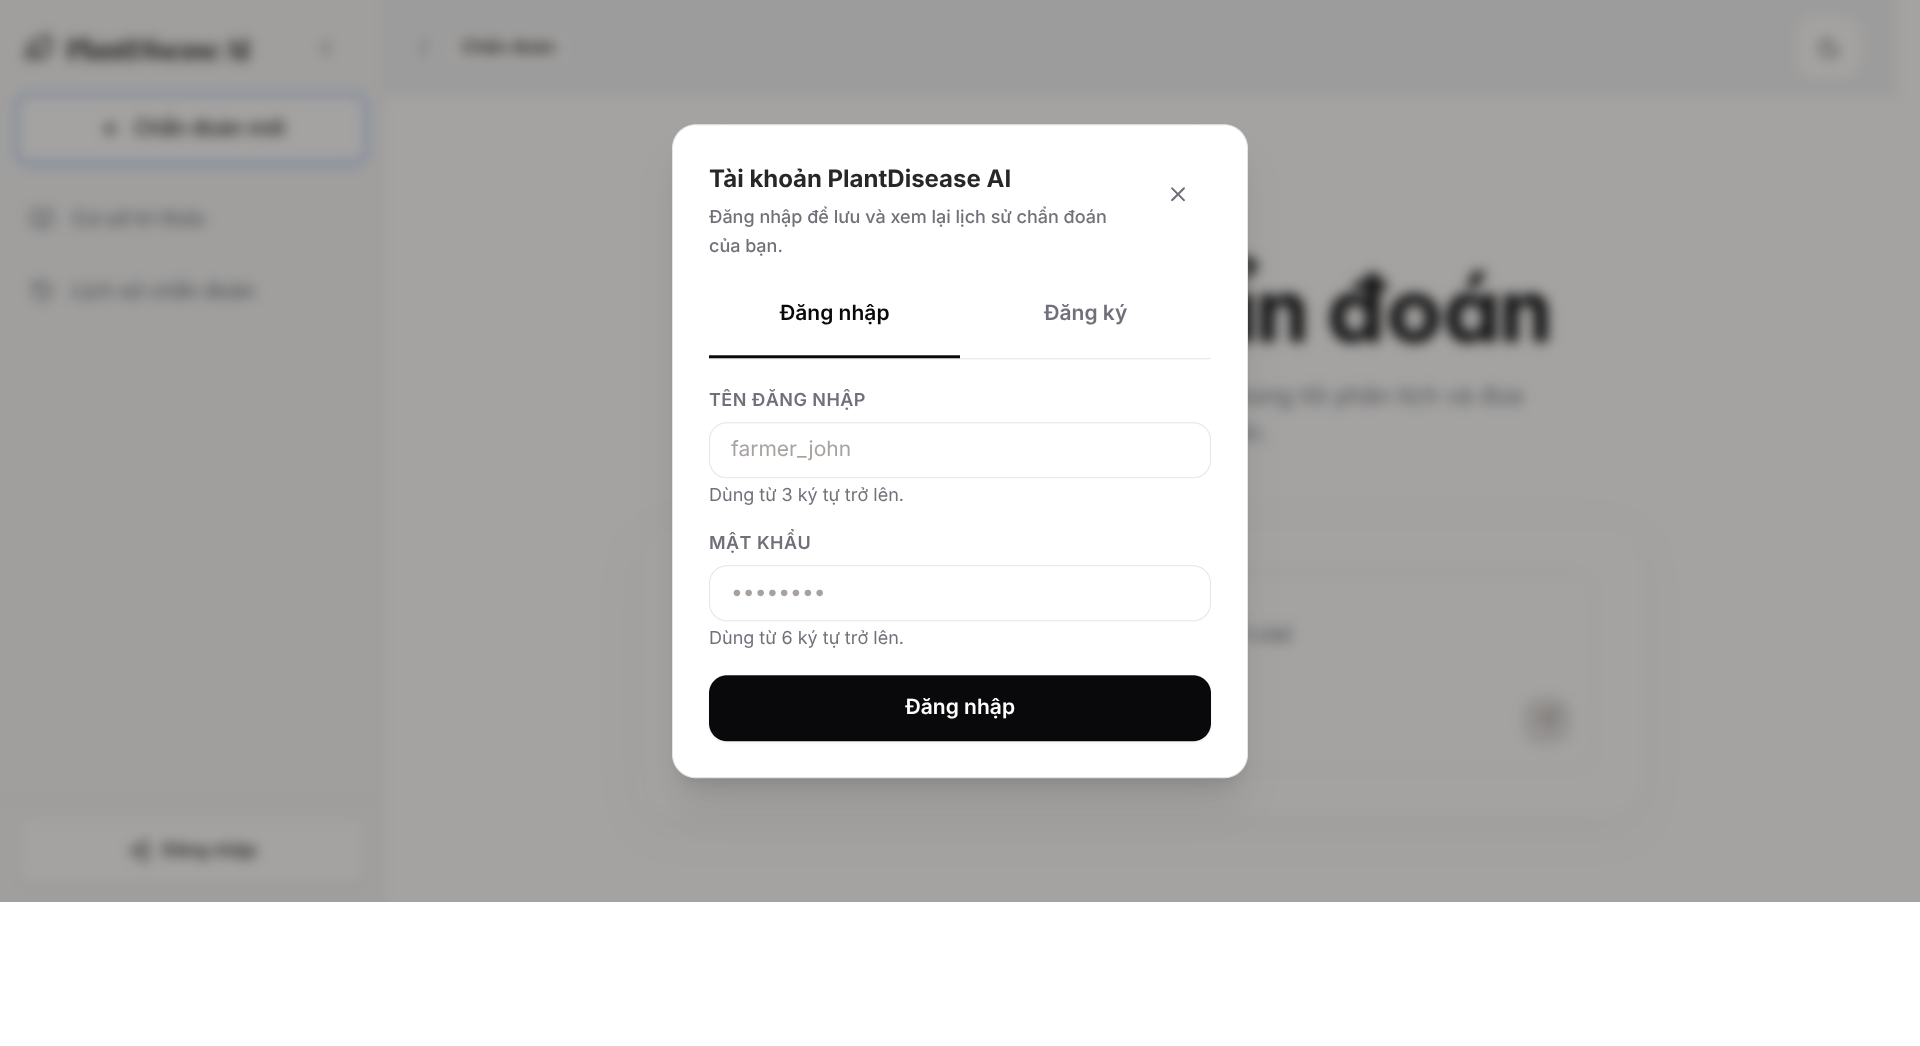
\includegraphics[width=\textwidth,height=0.72\textheight,keepaspectratio]{img/ch5/web-login.png}
  \caption{Giao diện đăng nhập để sử dụng lịch sử chẩn đoán}
  \label{fig:ch5-login}
\end{figure}

\subsubsection{Tải ảnh và chụp ảnh trực tiếp}

Ứng dụng cung cấp ba cách đưa ảnh lá cây vào luồng chẩn đoán: kéo--thả ảnh vào vùng nhập liệu, chọn tệp có sẵn bằng nút đính kèm, hoặc chụp ảnh mới bằng nút camera. Nút camera kích hoạt trường nhập ảnh với thuộc tính \texttt{capture="environment"}, nhờ đó trình duyệt trên thiết bị di động ưu tiên mở camera sau để người dùng hướng trực tiếp vào lá cây. Trên máy tính hoặc trình duyệt không hỗ trợ camera trực tiếp, hệ điều hành có thể chuyển về hộp thoại chọn tệp mà không làm gián đoạn luồng sử dụng.

Ảnh vừa chụp được xử lý giống ảnh tải lên: frontend kiểm tra định dạng JPEG, PNG hoặc WebP và giới hạn 10 MB, sau đó hiển thị ảnh thu nhỏ, tên tệp và dung lượng để người dùng xác nhận. Người dùng có thể xóa ảnh để chụp lại hoặc nhấn nút gửi để bắt đầu chẩn đoán. Trong Hình~\ref{fig:ch5-predict-coffee}, nút chụp ảnh mang biểu tượng camera nằm cạnh nút đính kèm ở cuối khung tải ảnh bên trái. Tính năng này đặc biệt phù hợp với bối cảnh sử dụng ngoài đồng ruộng, nơi người dùng thao tác chủ yếu bằng điện thoại và cần chẩn đoán ngay sau khi quan sát triệu chứng.

\subsubsection{Chẩn đoán và giải thích kết quả}

Tại màn hình chẩn đoán, người dùng tải ảnh hoặc chụp ảnh từ thiết bị, sau đó gửi yêu cầu đến backend. Kết quả hiển thị tên bệnh bằng tiếng Việt và tiếng Anh, cây trồng, mức độ, độ tin cậy, thời gian phản hồi và các lựa chọn khác của mô hình. Phần khuyến nghị trình bày mô tả, triệu chứng, nguyên nhân, biện pháp xử lý và phòng bệnh. Hình~\ref{fig:ch5-predict-coffee} minh họa một yêu cầu với ảnh lá cà phê; hệ thống nhận diện bệnh đốm rong, hiển thị top-$5$ và đồng thời cảnh báo vì độ tin cậy còn thấp. Cảnh báo này giúp tránh diễn giải xác suất dự đoán như một kết luận chuyên môn chắc chắn.

\begin{figure}[p]
  \centering
  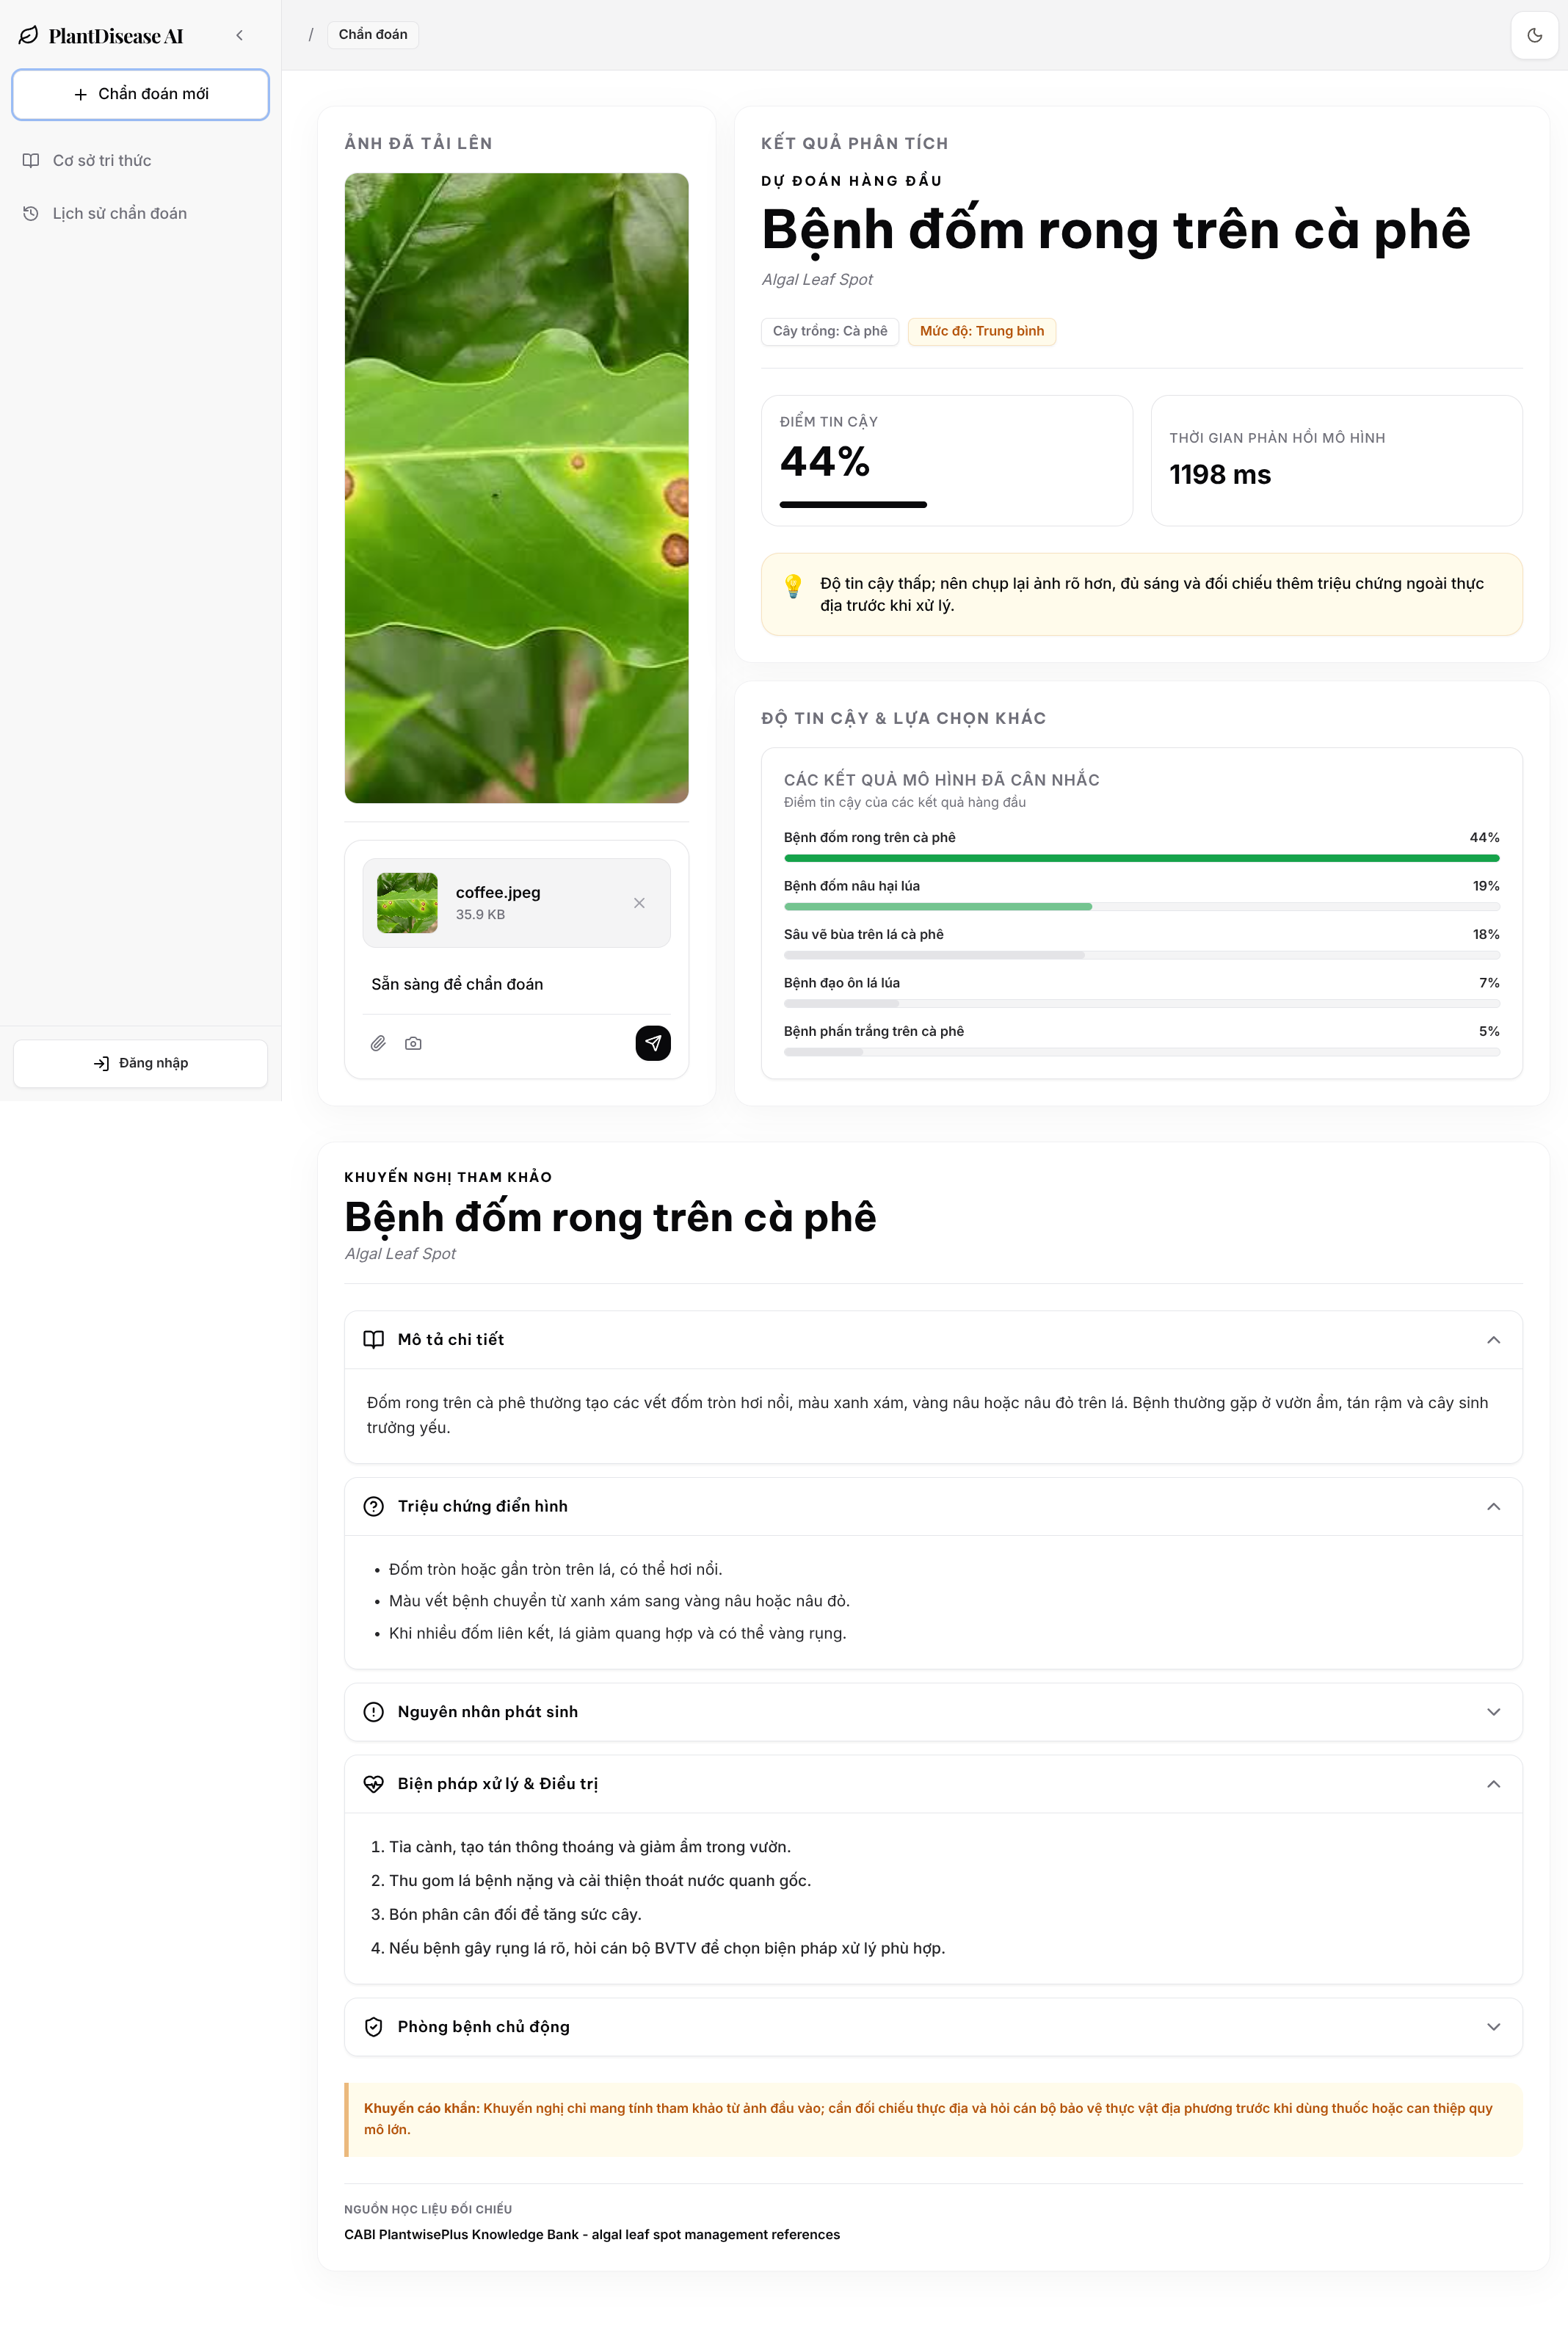
\includegraphics[height=0.88\textheight,keepaspectratio]{img/ch5/web-predict-coffee-v2.png}
  \caption{Kết quả chẩn đoán ảnh lá cà phê; khung bên trái hỗ trợ đính kèm hoặc chụp ảnh trực tiếp}
  \label{fig:ch5-predict-coffee}
\end{figure}

\subsubsection{Cơ sở tri thức chuyên gia}

Cơ sở tri thức cho phép tra cứu độc lập với thao tác dự đoán. Dữ liệu bao phủ tám nhãn mục tiêu của hai nhóm cây trồng và được kiểm tra tính đầy đủ khi backend nạp tệp. Mỗi bệnh có tên Việt--Anh, mức độ, mô tả, triệu chứng, nguyên nhân, biện pháp xử lý, phòng ngừa và nguồn đối chiếu. Hình~\ref{fig:ch5-knowledge} thể hiện danh sách và trang chi tiết. Nội dung luôn đi kèm lưu ý rằng khuyến nghị chỉ mang tính tham khảo và không thay thế đánh giá của cán bộ bảo vệ thực vật tại địa phương.

\begin{figure}[p]
  \centering
  \begin{subfigure}[t]{0.48\textwidth}
    \centering
    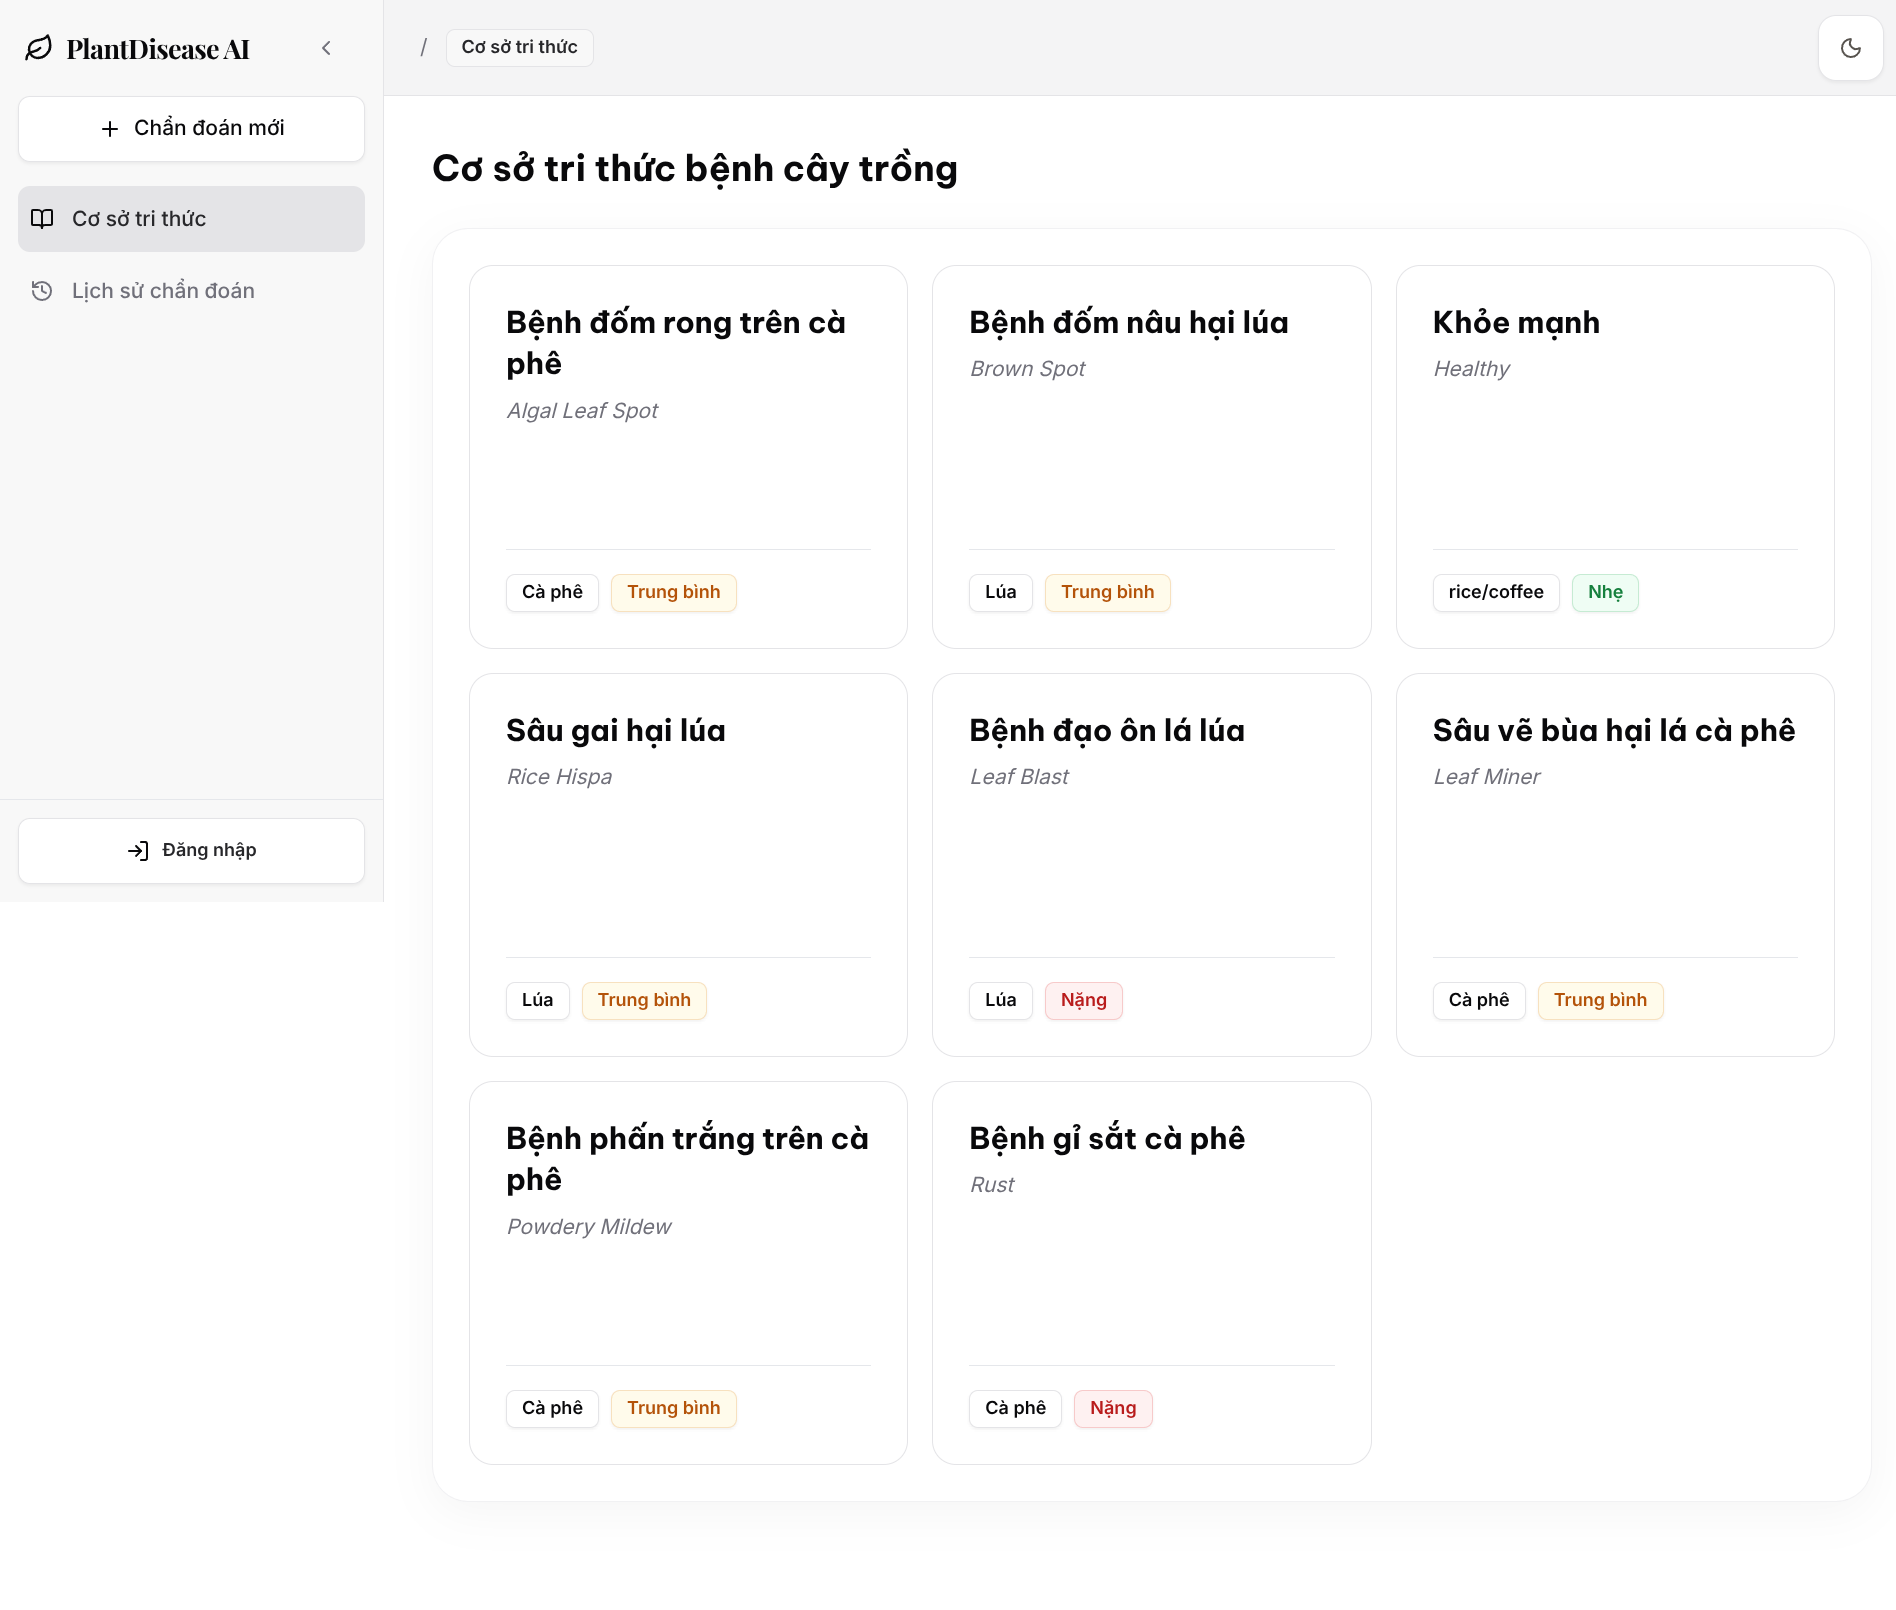
\includegraphics[width=\textwidth,height=0.77\textheight,keepaspectratio]{img/ch5/web-knowledge.png}
    \caption{Danh sách bệnh}
  \end{subfigure}
  \hfill
  \begin{subfigure}[t]{0.48\textwidth}
    \centering
    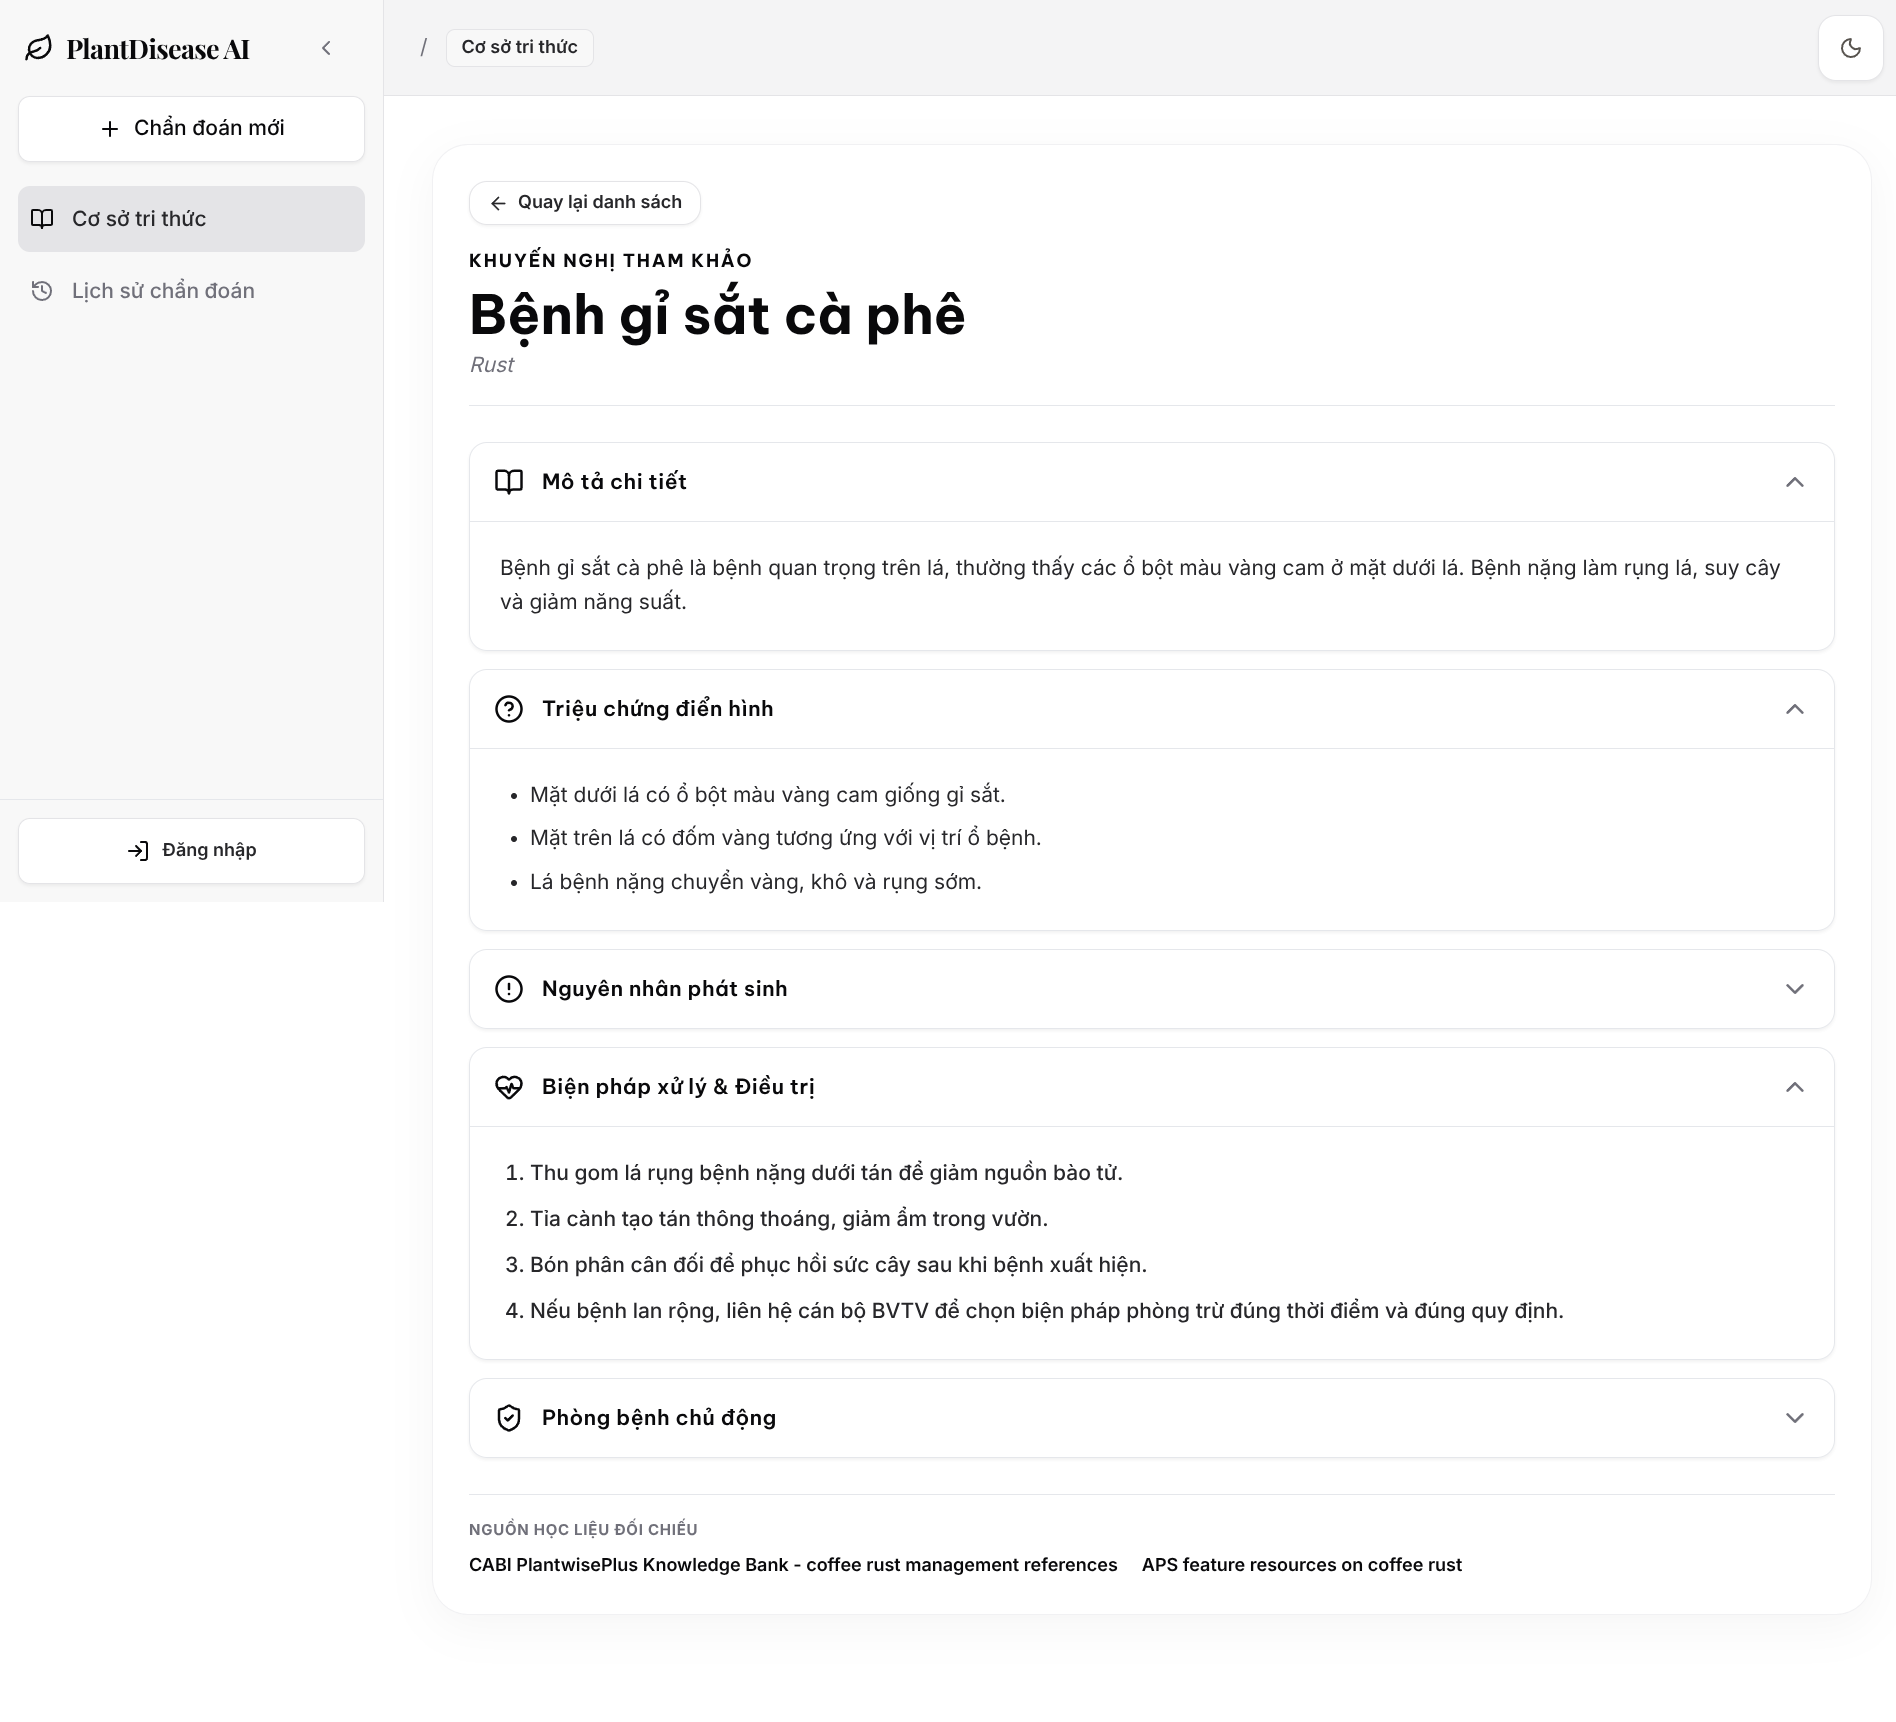
\includegraphics[width=\textwidth,height=0.77\textheight,keepaspectratio]{img/ch5/web-knowledge-detail.png}
    \caption{Thông tin chi tiết}
  \end{subfigure}
  \caption{Giao diện cơ sở tri thức bệnh trên lúa và cà phê}
  \label{fig:ch5-knowledge}
\end{figure}

\subsubsection{Tài liệu API}

FastAPI tự động sinh đặc tả OpenAPI và giao diện Swagger. Các nhóm endpoint gồm \textit{auth}, \textit{prediction}, \textit{history} và \textit{knowledge}; nhờ đó thành viên phát triển có thể kiểm tra schema yêu cầu, schema phản hồi và thử gọi API trực tiếp. Trên tên miền công khai đã nêu, Swagger được cung cấp tại đường dẫn \path{/docs} như minh họa trong Hình~\ref{fig:ch5-swagger}.

\begin{figure}[p]
  \centering
  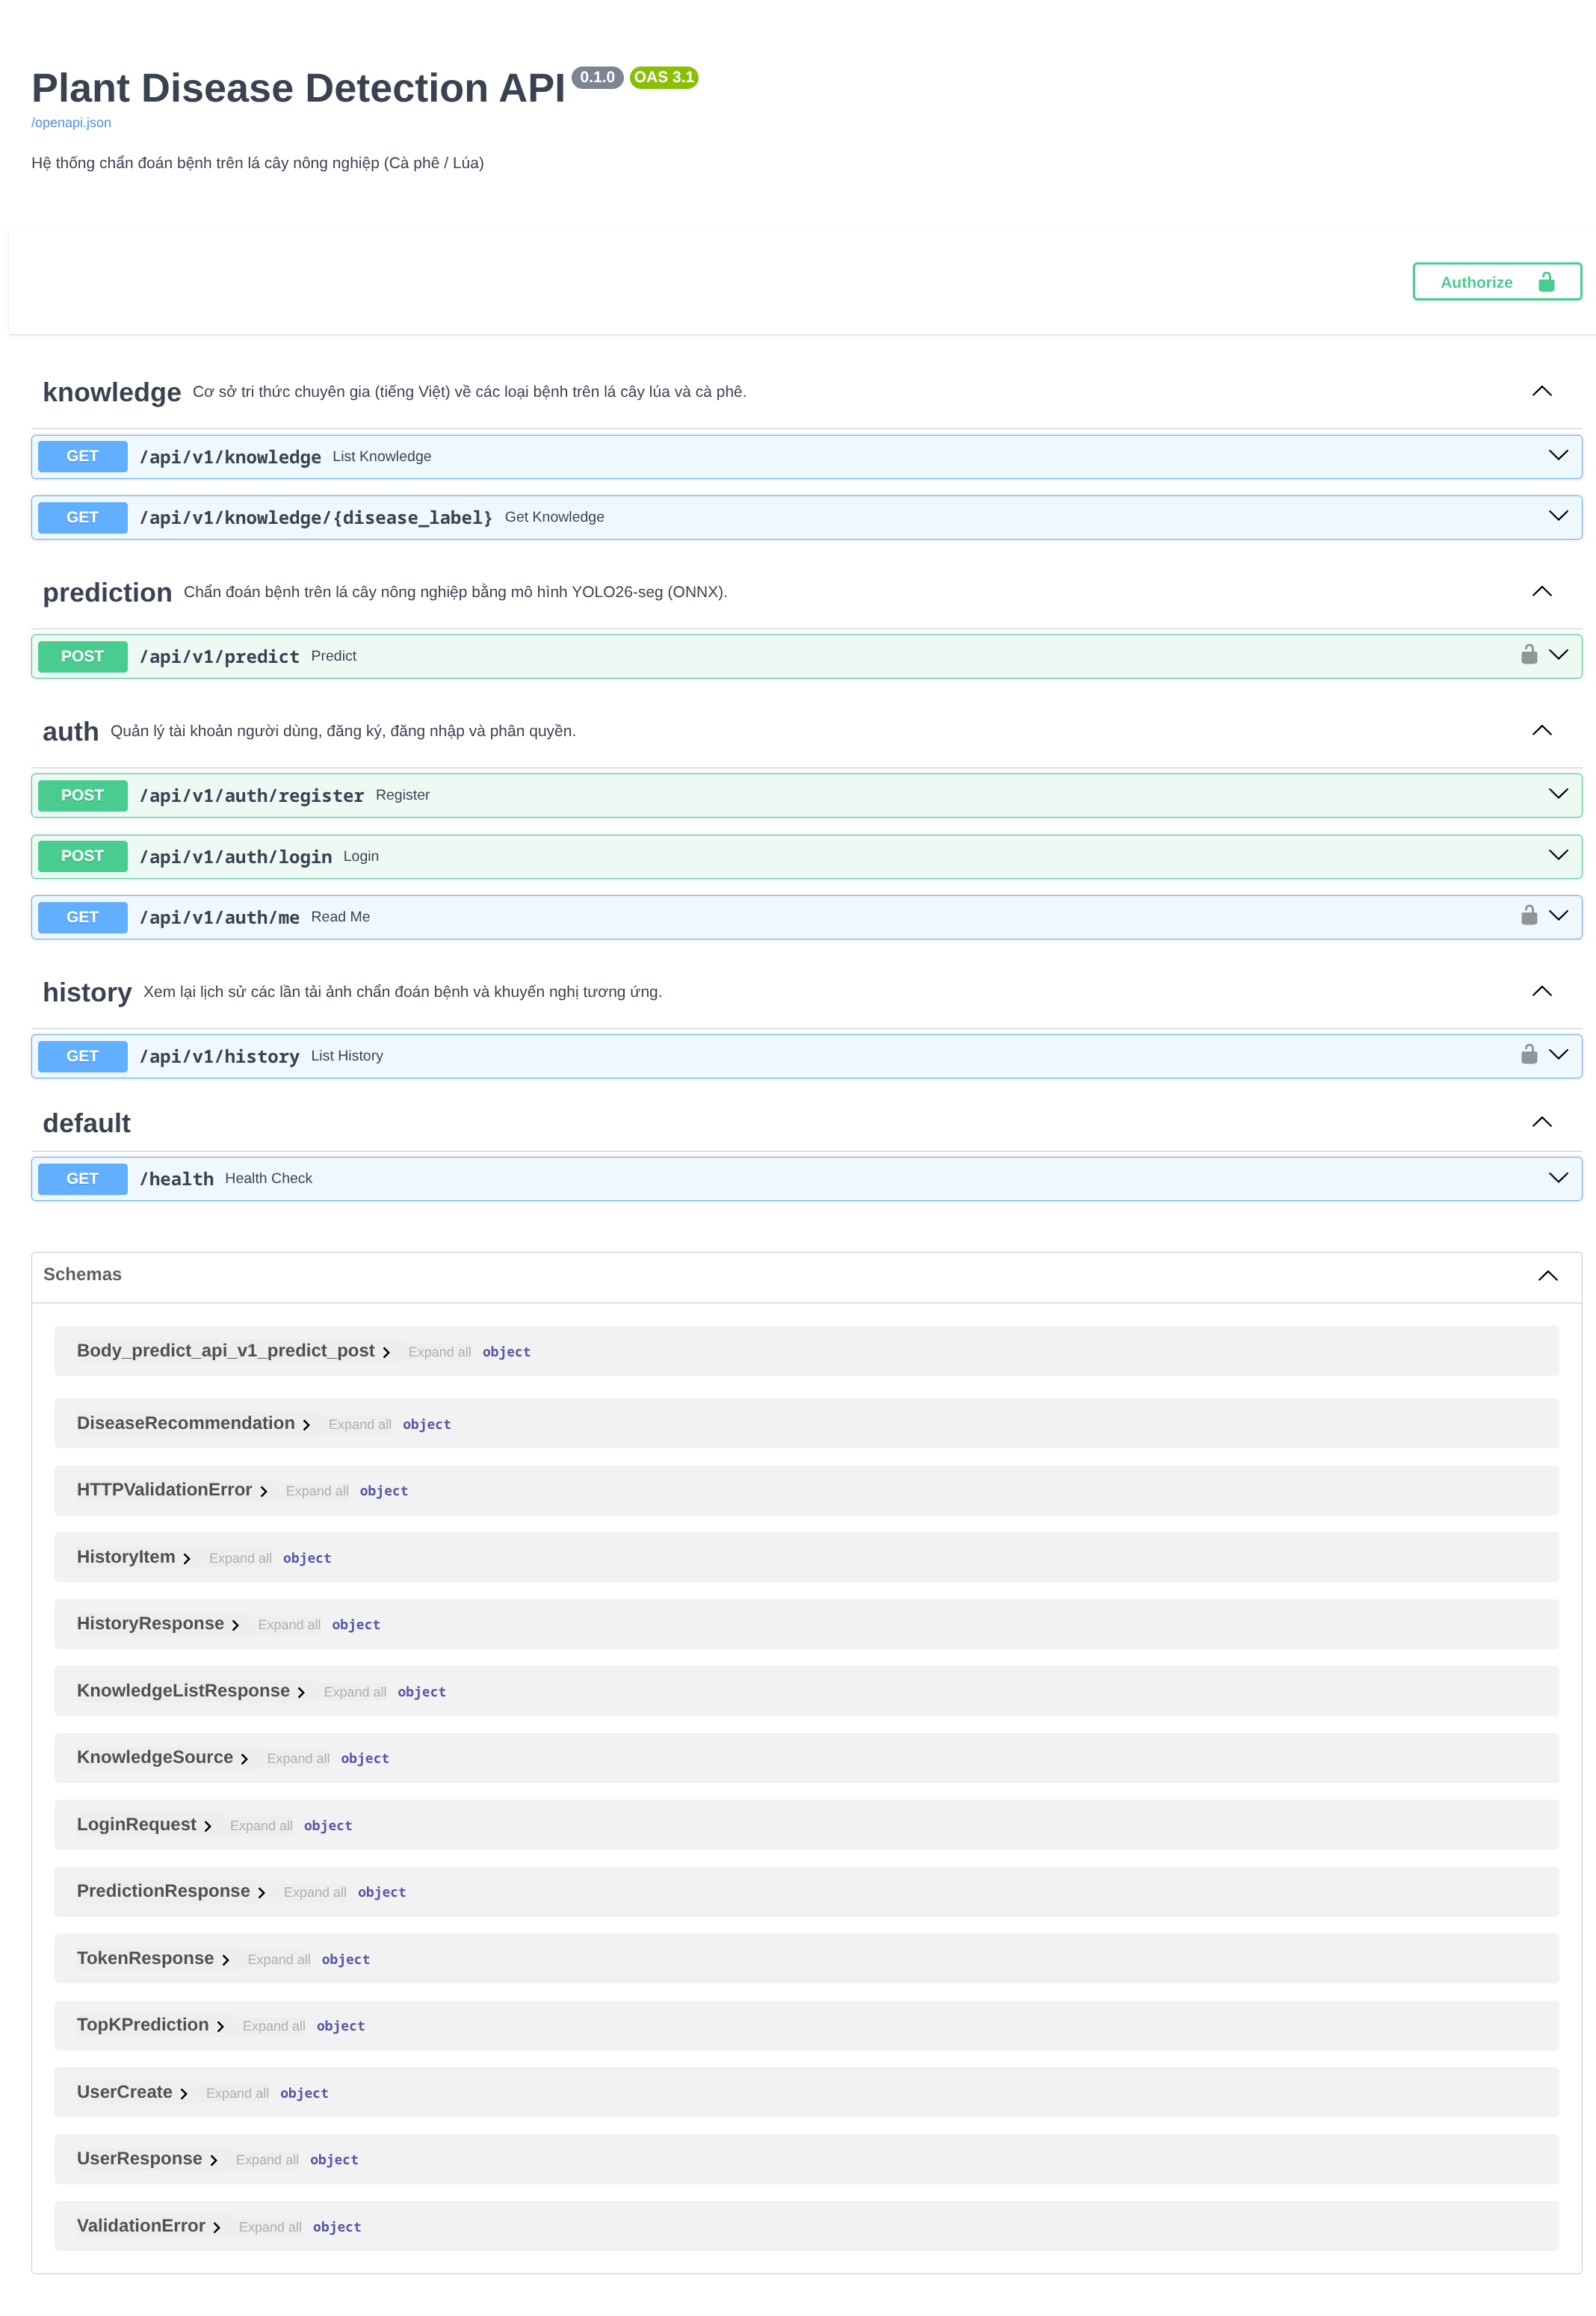
\includegraphics[height=0.86\textheight,keepaspectratio]{img/ch5/web-swagger.png}
  \caption{Tài liệu REST API trên Swagger UI}
  \label{fig:ch5-swagger}
\end{figure}

\FloatBarrier

\subsection{Triển khai trên GCP}

\subsubsection{Cụm k3s và Helm Chart}

Ứng dụng được triển khai trên một máy ảo Ubuntu 22.04 LTS của GCP. Thay vì sử dụng một dịch vụ Kubernetes được quản lý nhiều node, nhóm chọn k3s~\cite{k3s2026} để giảm chi phí tài nguyên và độ phức tạp vận hành của đồ án. Toàn bộ tài nguyên ứng dụng nằm trong namespace \texttt{plant-disease} và được quản lý bởi Helm release cùng tên. Helm Chart~\cite{helm2026} khai báo Deployment cho frontend/backend; StatefulSet cho PostgreSQL, MinIO và Redis; Service nội bộ; Ingress; Secret; PersistentVolumeClaim và CronJob sao lưu PostgreSQL.

Bảng~\ref{tab:ch5-k3s-workloads} tóm tắt cấu hình lưu trữ quan trọng. Các volume dùng chế độ \texttt{ReadWriteOnce}, phù hợp với cụm một node. PostgreSQL và MinIO được cấp volume lần lượt 20 GiB và 30 GiB; model dùng PVC 10 GiB; Redis dùng 1 GiB với cơ chế append-only. Ngoài ra, PostgreSQL được sao lưu định kỳ lúc 02:00 mỗi ngày và chính sách mặc định giữ bảy ngày.

\begin{table}[htbp]
  \centering
  \caption{Workload và lưu trữ trên cụm k3s}
  \label{tab:ch5-k3s-workloads}
  \small
  \begin{tabularx}{\textwidth}{|p{2.5cm}|p{2.5cm}|p{2.3cm}|X|}
    \hline
    \textbf{Workload} & \textbf{Kiểu tài nguyên} & \textbf{Lưu trữ} & \textbf{Dữ liệu chính} \\
    \hline
    Frontend & Deployment & Không & Production bundle Next.js, không giữ trạng thái. \\ \hline
    Backend & Deployment & Model PVC 10 GiB & Gắn read-only tại \texttt{/models} trong container chính. \\ \hline
    PostgreSQL & StatefulSet & 20 GiB & Tài khoản, metadata ảnh và lịch sử chẩn đoán. \\ \hline
    MinIO & StatefulSet & 30 GiB & Ảnh lá do người dùng tải lên. \\ \hline
    Redis & StatefulSet & 1 GiB & Hạ tầng cache/queue dự phòng cho giai đoạn mở rộng. \\ \hline
    PostgreSQL backup & CronJob & 5 GiB & Bản sao lưu định kỳ của cơ sở dữ liệu. \\ \hline
  \end{tabularx}
\end{table}

Mỗi container được giới hạn CPU và bộ nhớ để tránh một dịch vụ chiếm toàn bộ tài nguyên máy ảo. Backend được cấp tối đa 2 CPU và 6 GiB RAM do phải nạp mô hình; frontend tối đa 0,5 CPU và 512 MiB; ba dịch vụ dữ liệu có giới hạn nhỏ hơn. Secret sản xuất như khóa JWT, mật khẩu PostgreSQL và khóa MinIO không được ghi trực tiếp vào repository mà được truyền từ GitHub Actions khi chạy lệnh \texttt{helm upgrade --install}.

\subsubsection{Định tuyến, tên miền và HTTPS}

Tên miền DuckDNS \url{https://plant-disease-demo.duckdns.org/} trỏ đến địa chỉ công khai của máy ảo. Traefik là ingress controller mặc định của k3s và thực hiện định tuyến theo đường dẫn. cert-manager dùng ACME HTTP-01 với Let's Encrypt để cấp chứng chỉ cho secret \texttt{plant-disease-tls}. Nhờ đó, giao diện và API cùng được phục vụ qua HTTPS trên một tên miền, trong khi PostgreSQL, MinIO console và Redis không bị công khai.

\subsubsection{Quy trình CI/CD}

Workflow \texttt{deploy.yml} tự động hóa bốn giai đoạn nối tiếp:

\begin{enumerate}
  \item \textbf{Lint và kiểm thử:} cài dependency Python bằng \texttt{uv}, chạy bộ kiểm thử backend, cài dependency frontend và tạo production build.
  \item \textbf{Build và push:} dùng Docker Buildx để tạo image frontend/backend, gắn cả tag theo mã commit và \texttt{latest}, sau đó đẩy lên GitHub Container Registry (GHCR).
  \item \textbf{Deploy:} đóng gói Helm Chart, chuyển chart đến GCP VM qua SSH và chạy \texttt{helm upgrade --install}. Tag image được đặt bằng SHA của commit để mỗi lần triển khai có thể truy vết chính xác.
  \item \textbf{Smoke test:} chờ rollout, kiểm tra \texttt{/health}, cơ sở tri thức và luồng đăng ký tài khoản trên tên miền công khai. Bước dự đoán ảnh đầy đủ hiện vẫn được thực hiện thủ công vì workflow chưa đóng gói ảnh mẫu.
\end{enumerate}

Hình~\ref{fig:ch5-cicd} ghi nhận năm kiểm tra liên quan đến lint, test, build, deploy và smoke test đều hoàn tất thành công. Việc dùng chuỗi phụ thuộc giữa các job bảo đảm image chỉ được phát hành khi kiểm tra trước đó đã đạt yêu cầu.

\begin{figure}[htbp]
  \centering
  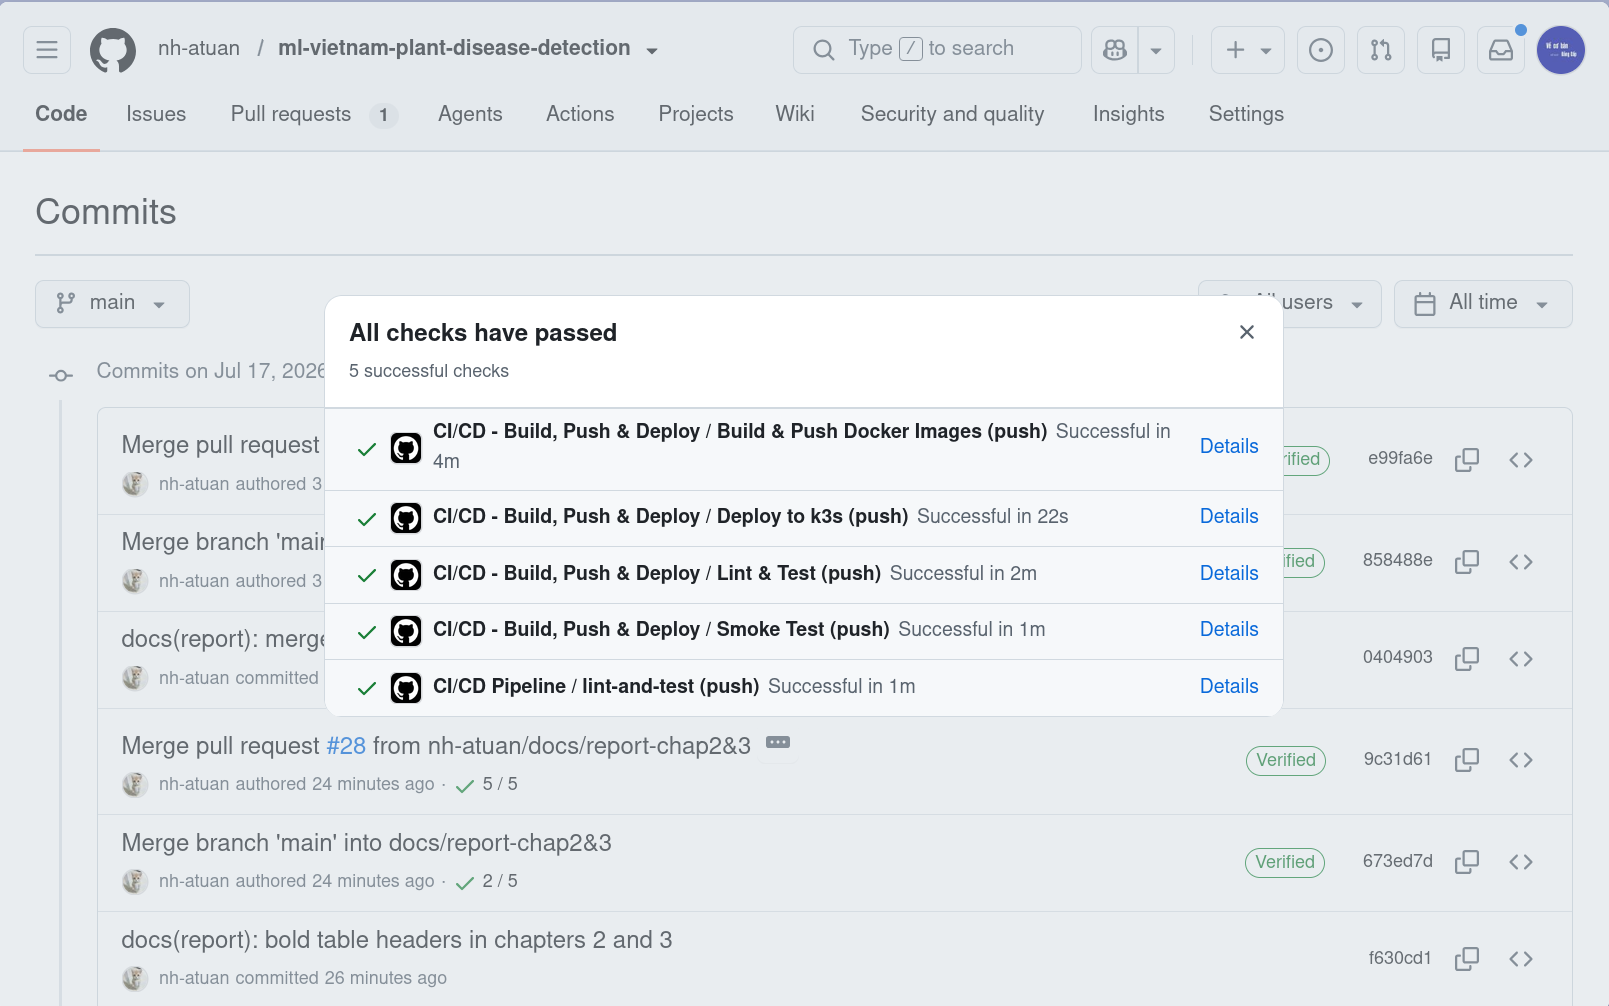
\includegraphics[width=\textwidth,height=0.75\textheight,keepaspectratio]{img/ch5/cicd-pipeline-success.png}
  \caption{Các bước CI/CD hoàn tất thành công trên GitHub Actions}
  \label{fig:ch5-cicd}
\end{figure}

\subsubsection{Minh chứng trạng thái vận hành}

Sau khi triển khai, nhóm kiểm tra node, pod, service, ingress, PersistentVolumeClaim và trạng thái Helm release bằng \texttt{kubectl} và \texttt{helm}. Kết quả tại thời điểm ghi nhận trong Hình~\ref{fig:ch5-kubernetes-status} cho thấy node \texttt{plant-demo-k3s} ở trạng thái \texttt{Ready}; các workload frontend, backend, PostgreSQL, MinIO và Redis ở trạng thái \texttt{Running}; các job sao lưu đã \texttt{Completed}; ingress công bố cổng 80/443; Helm release ở trạng thái \texttt{deployed}. Đây là bằng chứng trực tiếp rằng hệ thống không chỉ có cấu hình triển khai trong repository mà đã hoạt động trên hạ tầng cloud công khai.

\begin{figure}[H]
  \centering
  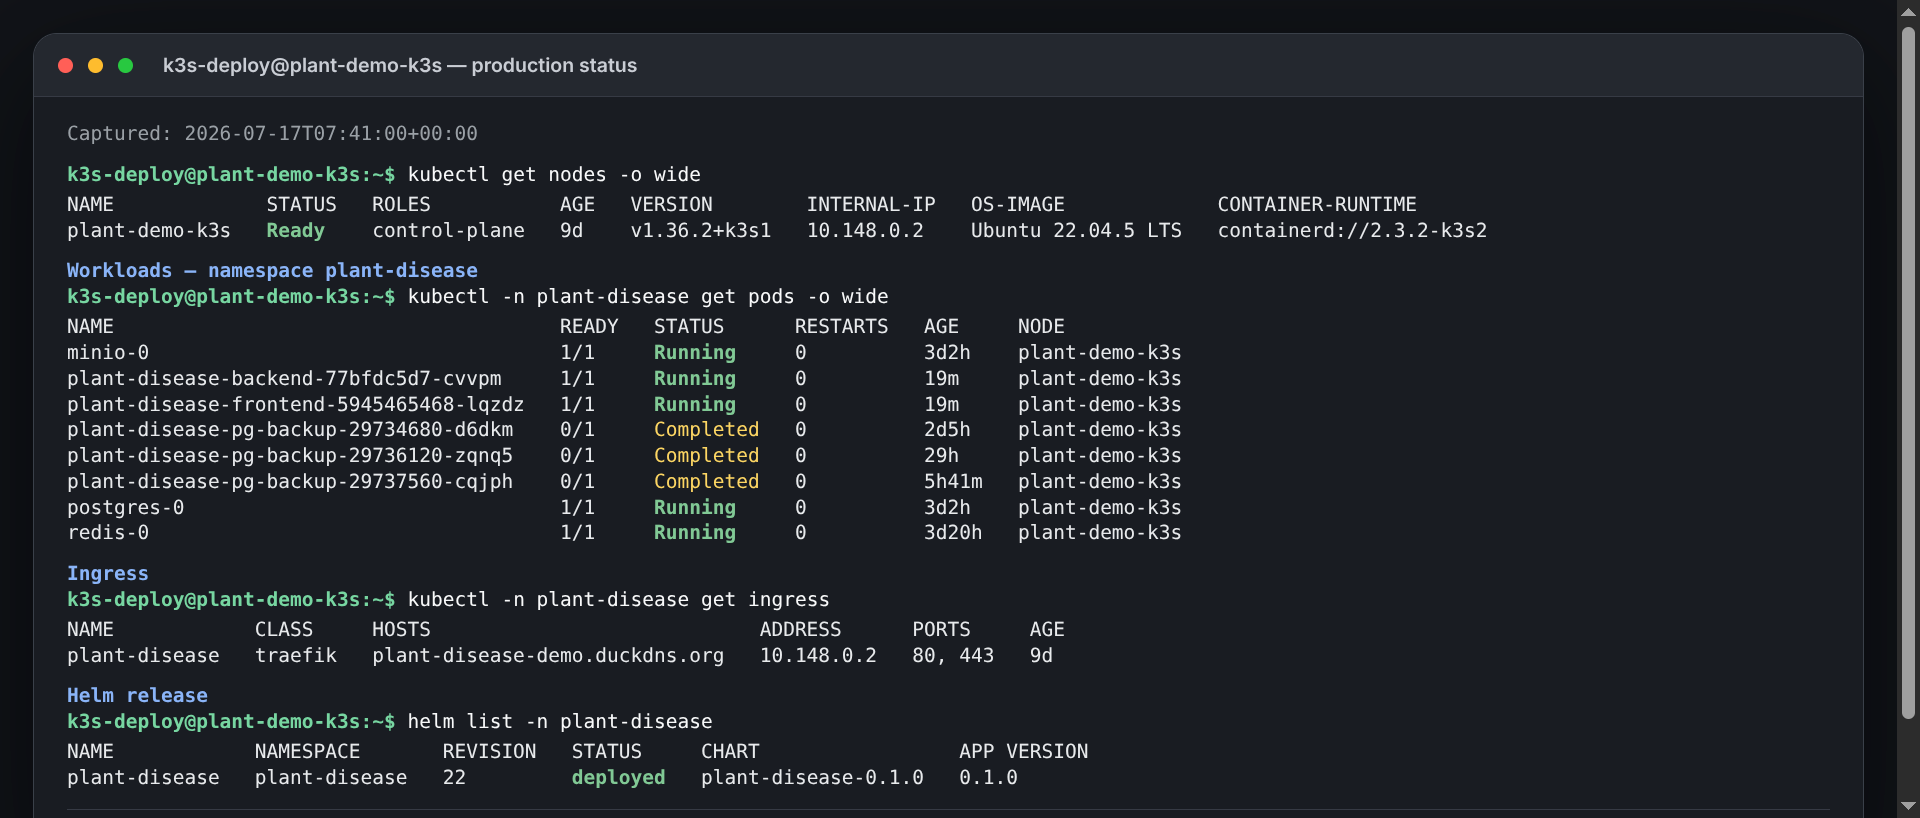
\includegraphics[width=\textwidth,height=0.82\textheight,keepaspectratio]{img/ch5/kubernetes-status.png}
  \caption{Trạng thái cụm k3s và Helm release trên GCP}
  \label{fig:ch5-kubernetes-status}
\end{figure}

\FloatBarrier

\subsection{Đánh giá và Giới hạn Triển khai}

Kết quả triển khai cho thấy chuỗi từ giao diện, REST API, mô hình ONNX, cơ sở tri thức, cơ sở dữ liệu và lưu trữ ảnh đã được tích hợp thành một sản phẩm có thể truy cập công khai. Việc sử dụng Docker, Helm và CI/CD giúp môi trường vận hành có khả năng tái lập tốt hơn so với cài đặt thủ công; readiness/liveness probe, lưu trữ bền vững và sao lưu PostgreSQL hỗ trợ duy trì dịch vụ khi pod được tạo lại.

Tuy nhiên, kiến trúc hiện tại vẫn có một số giới hạn. Cụm chỉ có một node nên máy ảo là điểm lỗi đơn; các volume \texttt{local-path} không cung cấp khả năng sao chép dữ liệu sang node khác; số replica frontend/backend hiện là một; model PVC cần được nạp artifact trước khi backend có thể suy luận; CORS của backend vẫn cho phép mọi origin; Redis chưa được tích hợp vào luồng nghiệp vụ; và smoke test tự động chưa bao phủ yêu cầu dự đoán ảnh đầu-cuối. Đây là các hướng ưu tiên nếu hệ thống được mở rộng ngoài phạm vi đồ án: chuyển sang cụm nhiều node và storage có replication, tăng số replica stateless, giới hạn CORS theo tên miền, tự động hóa phân phối model, bổ sung quan sát hệ thống và đưa ảnh mẫu hợp lệ vào smoke test.
